\section{Update}
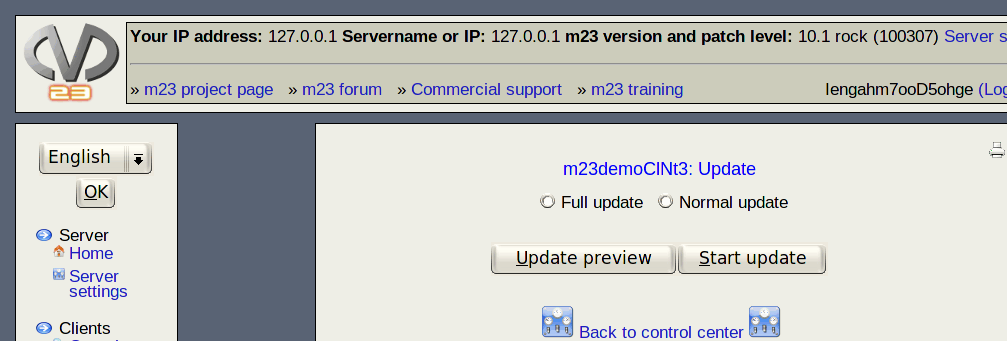
\includegraphics[scale=0.4]{/mdk/doc/manual/screenshots/de/update_packages.png} \\
Mit der Update-Funktion k�nnen Sie die Software auf dem/den Client(s) updaten. Wenn Sie einen einzelnen Client ausgew�hlt haben, k�nnen Sie sich eine Update-Vorschau zeigen lassen.\\
\subsection{Update-Typen}
\begin{itemize}
\item \textbf{Normal-Update:} Updatet vorhandene Pakete und installiert nur neue Pakete, wenn diese unbedingt ben�tigt werden.\\
\item \textbf{Komplett-Update:} Vorhandene Pakete werden geupdatet, sowie neue Pakete installiert und ggf. alte entfernt.\\
\end{itemize}
